\documentclass[10pt, t]{beamer}
% \usepackage[UTF8]{ctex}
\usepackage{amsmath}
\usepackage{setspace}
\usepackage{float} 
\usepackage{multido}
\usepackage{multirow}
\usepackage{array}
\usepackage{enumerate}
\usepackage{booktabs}
\usepackage{indentfirst} 
\usepackage[style=mla]{biblatex}
\usepackage{setspace}
\usepackage{subcaption}
\usepackage{hyperref}
\usepackage{textpos}
% \usepackage{fontspec}

% \beamerdefaultoverlayspecification{<+->}
\makeatletter
\let\@@magyar@captionfix\relax
\makeatother

\definecolor{bladerunnerblue}{RGB}{41, 159, 163}
\definecolor{bladerunnerred}{RGB}{194,84,97}
\definecolor{themecolor}{RGB}{25,25,112} 
\definecolor{weak}{RGB}{150,150,150}

\renewcommand{\emph}[1]{{\color{themecolor}\textsl{#1}}}
\newcommand{\alarm}[1]{{\color{bladerunnerred}{#1}}}
\newcommand{\N}{\mathbb{N}}
\newcommand{\R}{\mathbb{R}}
\newcommand{\dom}{\operatorname{dom}}
\newcommand{\myseries}[2]{$#1_1,#1_2,\dots,#1_#2$}
\newcommand{\nullspace}{~\\[15pt]}
\newcommand{\remark}{\textbf{Remark: }}
\newcommand{\question}{\textbf{Question: }}
\newcommand{\scp}[2]{\langle\,#1\,,\,#2\,\rangle} \newcommand{\scpp}{\langle\,\cdot\,,\,\cdot\,\rangle}
\newcommand{\weaken}[1]{{\color{weak}\textit{#1}}}
\newcommand{\underover}[3]{\underset{#2}{\overset{#3}{#1}}}
\renewcommand{\emptyset}{\varnothing}


\usetheme{Madrid}
\setbeamertemplate{navigation symbols}{}

\addtobeamertemplate{frametitle}{}{
\begin{textblock*}{100mm}(0.85\textwidth,-1cm)
\includegraphics[height=1cm]{../../logo.png}
\end{textblock*}}


\usecolortheme[named=themecolor]{structure}

\setbeamertemplate{items}[default]

\hypersetup{
    colorlinks=true,
    linkcolor=themecolor,
    filecolor=themecolor,      
    urlcolor=themecolor,
    citecolor=themecolor,
}

\title{VV186: Honors Mathematics}
\subtitle{Functions \& Differentiation}
\institute[UM-SJTU JI]{Univerity of Michigan-Shanghai Jiao Tong University Joint Institute}
\author{Xingjian Zhang}

\begin{document}

\begin{frame}
    \titlepage
    \begin{center}
        \includegraphics[height=2cm]{../../logo2.png}
    \end{center}
\end{frame}

\begin{frame}
    \frametitle{RC Policy}
    Several things I want you to pay attention to:
    \begin{enumerate}
        \item \alarm{Be interactive.} Feel free to interrupt me at any time if you want to ask something or simply make some comments. You are free to discuss with your friend if you want, as long as your discussion is related to the course contents and your voice won't effect other students.
        \item Speak everything in \alarm{English} during the RC. This might be hard at the beginning, but you will soon get used to that.
        \item \alarm{``Question everything.''} Do not pretend to have understood everything. Maths is about strictness, abstraction and generalization. Understanding every basic concept is essential in our course. I will be quite ``push'' on checking your conceptual understanding. This process will be \textbf{annoying, tedious, but rewarding}. So Get prepared.
    \end{enumerate}
\end{frame}

\begin{frame}
    \frametitle{Outline}
    \begin{spacing}{1}
        \tableofcontents
    \end{spacing}
\end{frame}

\section{Assignment}
\begin{frame}
    \frametitle{Assignment 4}
    \begin{enumerate}
        \item Feedback is posted on \href{https://piazza.com/class/kdvbtz3cxva7mb?cid=79}{VV186 Piazza - Feedback for Assignment 4}.
        \item Come to OH if you have further questions.
    \end{enumerate}
\end{frame}

\section{Functions}
\subsection{Landau Symbol}
\begin{frame}
    \frametitle{Landau Symbol}
    \begin{figure}[H]
        \centering
        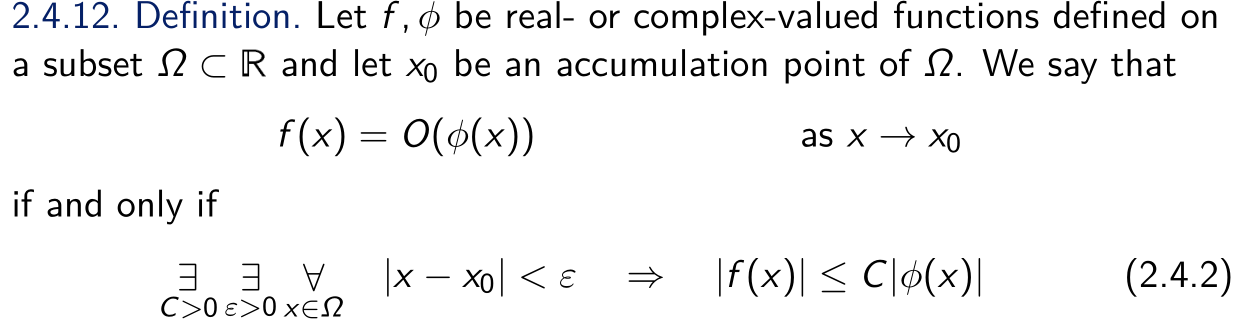
\includegraphics[width=0.9\textwidth]{2020-10-28-00-07-47.png}
    \end{figure}
    \begin{figure}[H]
        \centering
        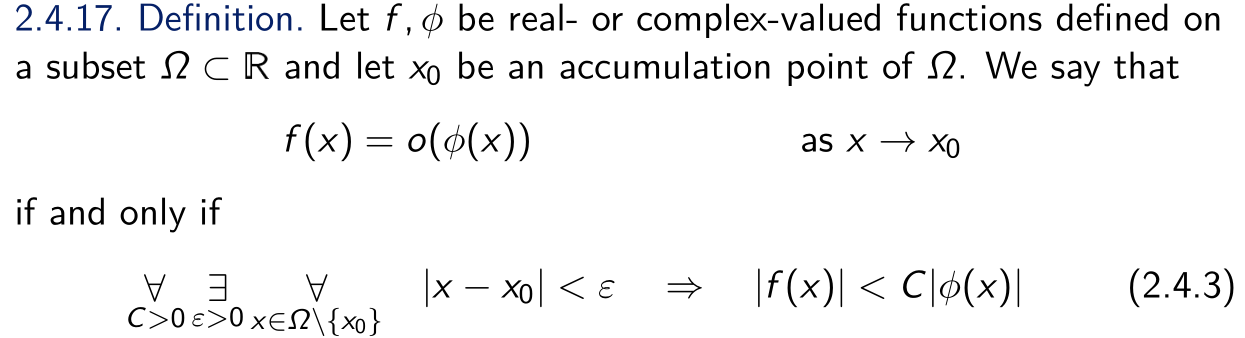
\includegraphics[width=0.9\textwidth]{2020-10-28-00-08-07.png}
    \end{figure}
\end{frame}

\begin{frame}
    \frametitle{Landau Symbol}

    \textbf{Remark:}
    \begin{enumerate}
        \item
              An intuitive interpretation of big- and small-O symbol:
              \begin{itemize}
                  \item $f(x)=O(g(x))$ as $x\to x_0$: $f(x)$ is not significantly greater than $g(x)$ as $x\to x_0$.
                  \item $f(x)=o(g(x))$ as $x\to x_0$: $f(x)$ is significantly less than $g(x)$ as $x\to x_0$.
              \end{itemize}
        \item Big-O symbol is very common in computer science. You will encounter it frequently in VE203, VE280, VE281, VE477 ...
        \item Small-O symbol is very common in our course (e.g. derivative).
        \item Notice that when $x_0=\infty$, the definition needs to be adjusted.
        \item We cannot know the exact behavior of a function from Landau notation.
    \end{enumerate}
\end{frame}

\begin{frame}
    \frametitle{Sufficient Condition of big O}

    \begin{figure}[H]
        \centering
        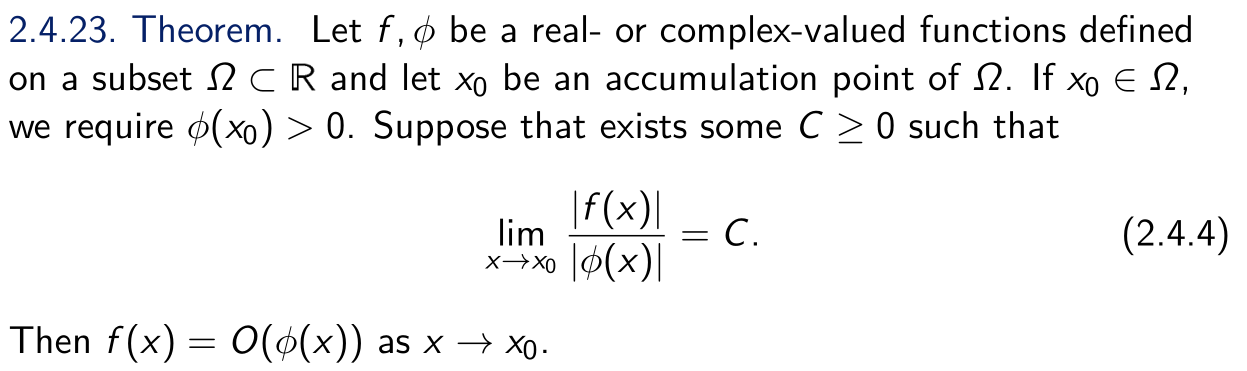
\includegraphics[width=0.9\textwidth]{2020-10-28-00-20-26.png}
    \end{figure}
    \textbf{Remark:} This theorem is useful when $(2.4.4)$ exists. However, one can still have $f(x)=O(\phi(x))$ as $x\to x_0$ even if it does not exist. *The requirement that $\phi(x_0)>0$ is a convention made by Landau.
\end{frame}

\begin{frame}
    \frametitle{Equivalent Condition of Small O}

    \begin{figure}[H]
        \centering
        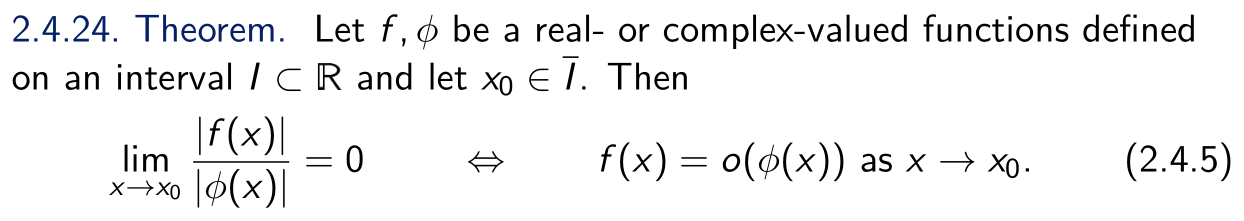
\includegraphics[width=0.9\textwidth]{2020-10-28-01-02-50.png}
    \end{figure}
    \textbf{Remark:} Notice that this theorem is a sufficient and necessary condition. With $f(x)=o(g(x))$ as $x\to x_0$, we cannot conclude that $f(x)\to 0$ as $x\to x_0$. A counter example is: $f(x)=1,g(x)=\frac{1}{|x|},x_0=0$.
\end{frame}

\begin{frame}
    \frametitle{Common Results}

    \begin{figure}[H]
        \centering
        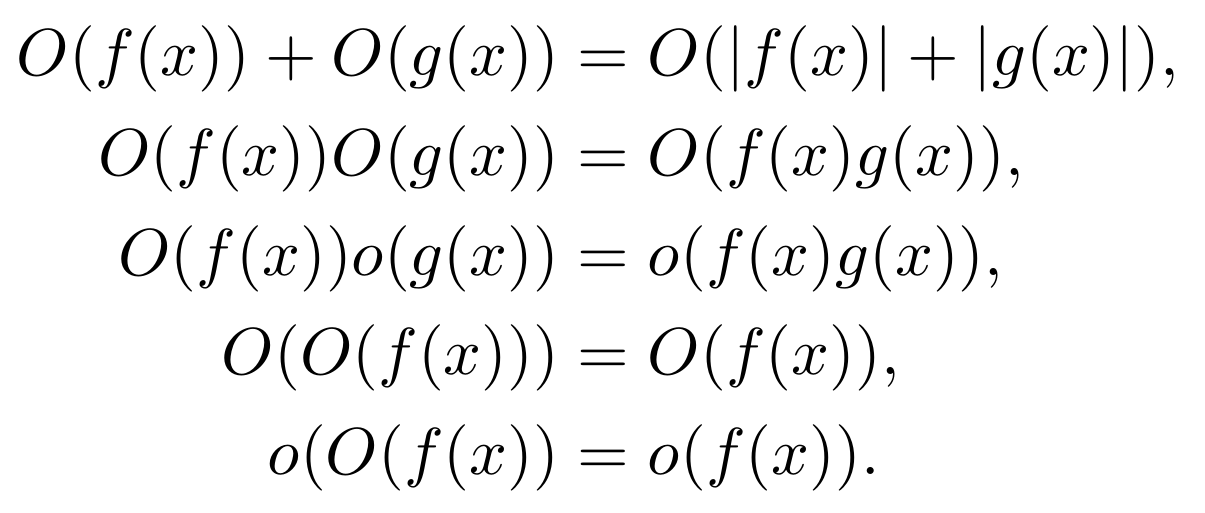
\includegraphics[width=0.6\textwidth]{2020-10-28-09-52-45.png}
    \end{figure}
\end{frame}

\subsection{Continuity}
\begin{frame}
    \frametitle{Continuity}
    \begin{figure}[H]
        \centering
        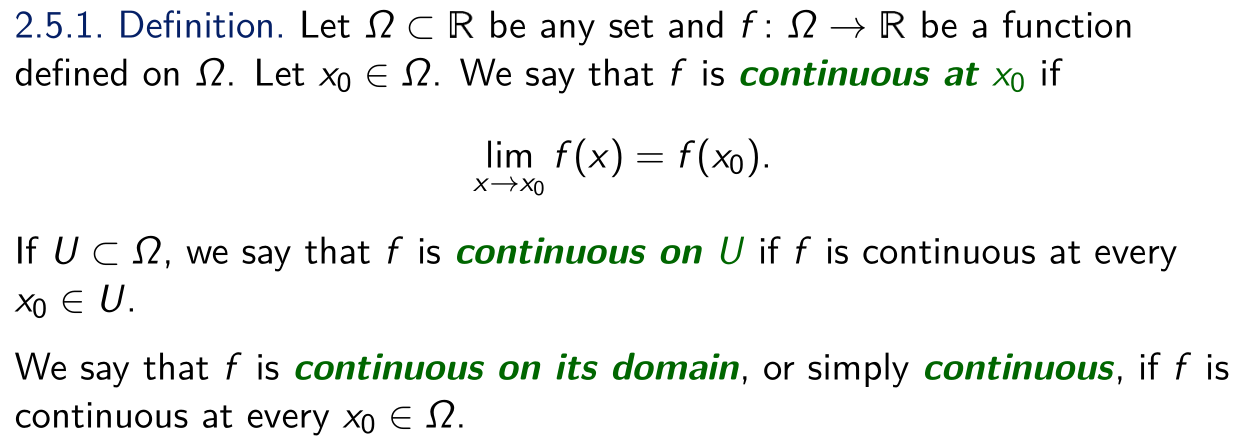
\includegraphics[width=0.9\textwidth]{2020-10-28-09-59-20.png}
    \end{figure}
    \question What are the three requirements of continuity?
\end{frame}

\begin{frame}
    \frametitle{Continuity}

    \begin{figure}[H]
        \centering
        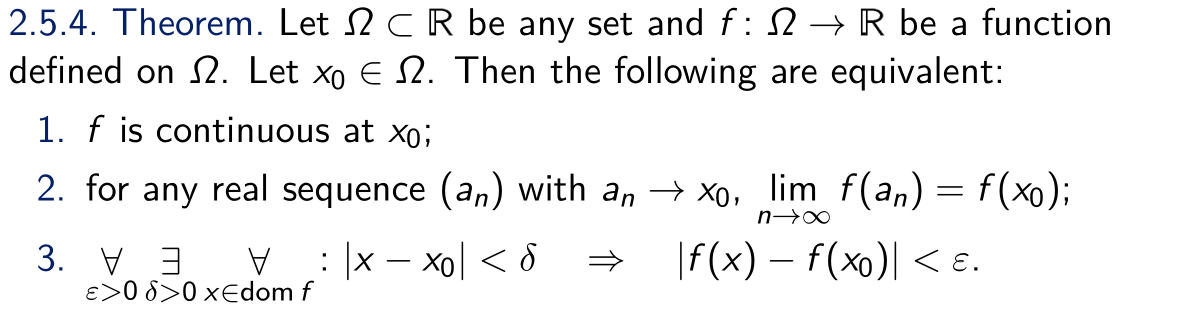
\includegraphics[width=0.9\textwidth]{2020-10-28-10-02-38.png}
    \end{figure}

\end{frame}

\begin{frame}
    \frametitle{Continuity: Composition of Functions}

    \begin{figure}[H]
        \centering
        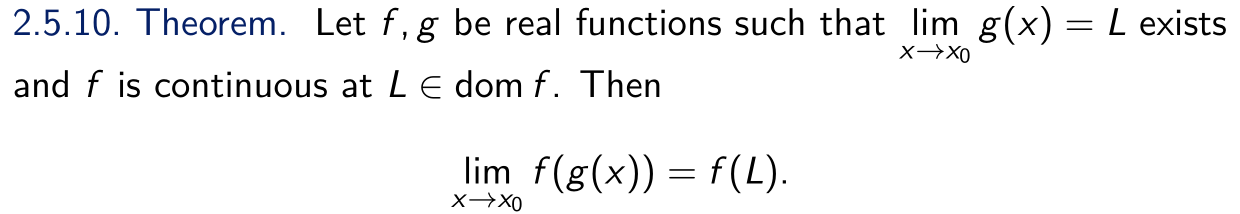
\includegraphics[width=0.9\textwidth]{2020-10-28-10-10-08.png}
    \end{figure}
    \pause
    \textbf{Proof: } \\
    Given $\varepsilon>0$. Since $f$ is continuous at $L$, $\exists \delta>0$ such that $\forall y\in \dom f: |L-y|<\delta\Rightarrow |f(L)-f(y)|<\varepsilon$.\\[10pt]
    We fix such $\delta>0$. Since $\underset{x\to x_0}{\lim}g(x)=L$, there is some $\tilde\delta>0$ such that $\forall x\in \dom g: |x_0-x|<\tilde\delta\Rightarrow |L-g(x)|<\delta\Rightarrow|f(L)-f(g(x))|<\varepsilon$.
\end{frame}

\begin{frame}
    \frametitle{Useful Results regarding Continuity}

    \begin{enumerate}
        \item Locally sign-preserving property (2.5.11. Lemma)
        \item The Bolzano Intermediate Value Theorem (2.5.12 \& 13. Theorem)
        \item Fixed Point Theorem (2.5.14. Theorem) \footnote[frame]{\textit{* Fixed point theorem} is a very powerful tool. For example, in VE203, we will prove bi-directional injection leads to a bijection between two sets using it.}
        \item Locally boundedness (2.5.15. Lemma)
        \item Globally boundedness on closed intervals (2.5.16. Proposition)
        \item Existence of global extrema on closed intervals (2.5.17. Theorem)
    \end{enumerate}
    \textbf{Remark:} Remember these results. They are useful in proof, and help you get a better sense towards continuity.
\end{frame}

\begin{frame}
    \frametitle{Exercise}

    1. Assume $f\in C([0,2a]),\, a>0,\, f(0)=f(2a).$\footnote[frame]{ $C(I)$ denotes the set of all continuous function on $I$.} Prove that there exists some $\zeta \in [0,a]$ such that $f(\zeta)=f(\zeta +a)$.\\
    \vspace{30pt}
    2. Let $f:[0,+\infty)\to \R$ be a continuous function such that $\underset{x\to\infty}{\lim}f(x)<\infty$ exists. Show that $f$ is uniformly continuous on its domain.
\end{frame}

\subsection{Inverse Functions}
\begin{frame}
    \frametitle{Inverse Functions}
    \begin{figure}[H]
        \centering
        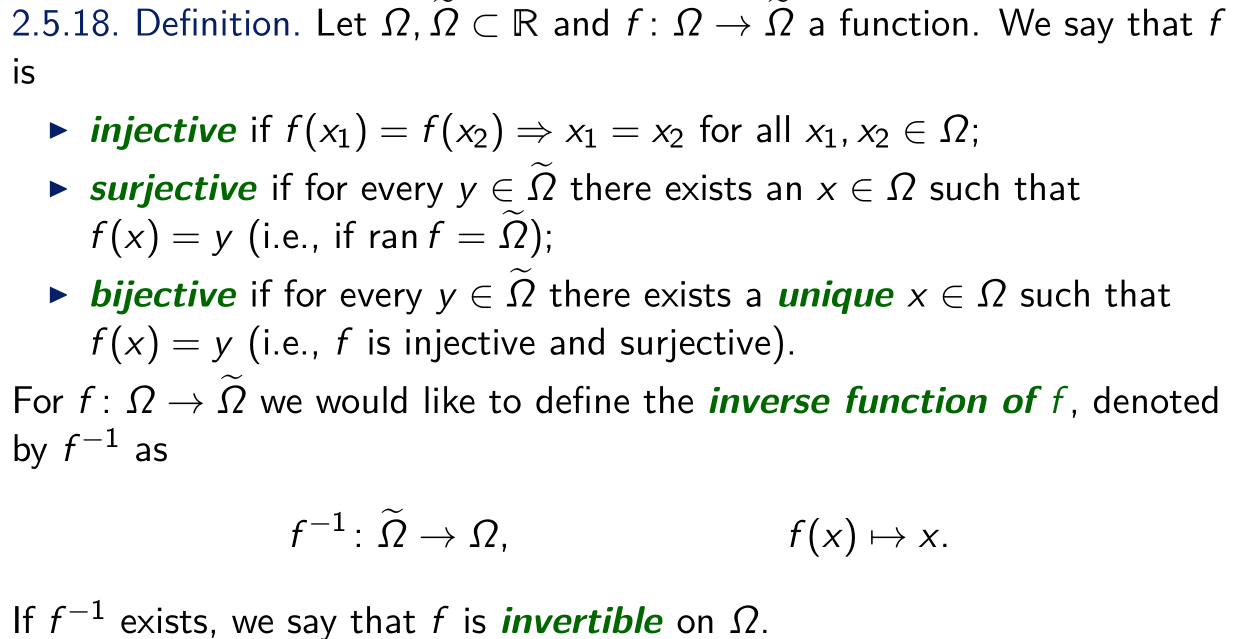
\includegraphics[width=0.9\textwidth]{2020-10-28-11-06-58.png}
    \end{figure}
    \textbf{Remark:}
    \begin{itemize}
        \item
              If $f$ is bijective, $f^{-1}$ exists.
        \item A continuous strictly monotonic function on an interval is bijective.
        \item A continuous bijective function on an interval is strictly monotonic.
    \end{itemize}
\end{frame}

\begin{frame}
    \frametitle{Image and Pre-Image of Sets}

    Write down the definition of them from memory.
    \pause
    \begin{figure}[H]
        \centering
        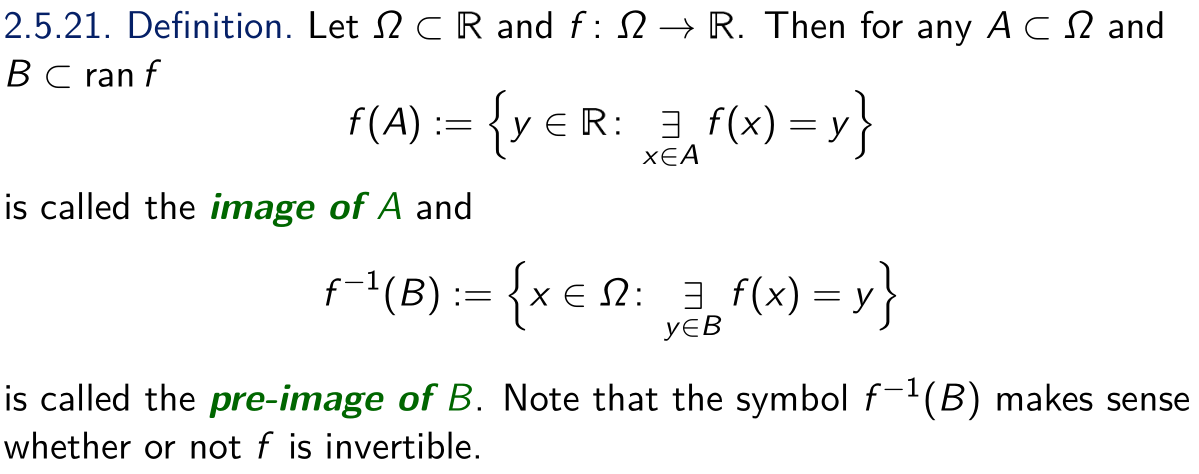
\includegraphics[width=0.9\textwidth]{2020-10-28-12-26-27.png}
    \end{figure}
    \textbf{Remark:}
    \begin{itemize}
        \item
              $f(\dom f)=\operatorname{ran} f$.
        \item $f^{-1}(\operatorname{ran} f)=f(\dom f)$.
    \end{itemize}
\end{frame}

\subsection{Uniform Continuity}
\begin{frame}
    \frametitle{Uniform Continuity}

    \begin{figure}[H]
        \centering
        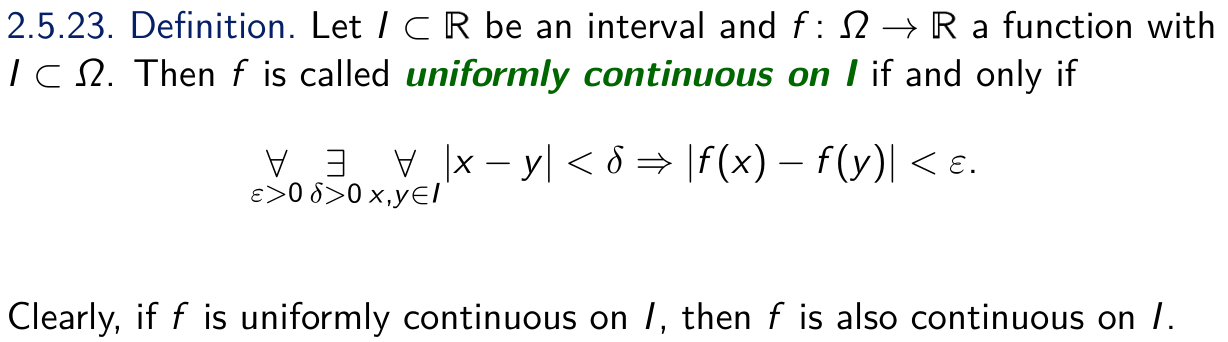
\includegraphics[width=0.9\textwidth]{2020-10-28-12-30-39.png}
    \end{figure}
    \textbf{Remark:} \\$f$ is uniformly continuous on $I$ $\Leftrightarrow$ $f$ is continuous on $I$\\ where $I=[a,b]\subset \dom f$. However,
        If $I$ is not closed, they are not equivalent any more.
\end{frame}

\begin{frame}
    \frametitle{Recall...}
    Are the following functions continuous? uniformly continuous?
    \begin{itemize}
        \item $f(x)=1/x$ on $(0,1)$
        \item $f(x)=1/x$ on $(1,2)$
        \item $f(x)=1/(1+x^2)$ on $\R$
        \item $f(x)=x$ on $\R$
        \item $f(x)=x^2$ on any bounded interval $I\subset \R$
        \item $f(x)=x^2$ on $\R$
    \end{itemize}
    What is the similarity and difference between continuity and uniform continuity?
\end{frame}

\section{Differential Calculus}
\subsection{``Linear Approximation''}
\begin{frame}
    \frametitle{``Linear Approximation''}

    We all learned \emph{differential calculus} in our high school but we usually called it \emph{``derivative''}. It was often defined in a sloppy way, and lacking of mathematical interpretation. At this moment, we want to formulate a strict definition of \emph{derivative} and \emph{differentiation}. With this solid, scalable definition, we can easily extend the derivative to higher-dimension space\footnote[frame]{We will cover them in VV285, where you will know matrices are derivatives of  multi-variable functions. At then, you may not be very surprised by this result if you understand the essence of derivate -- it is simply linear approximation.}.
    \nullspace
    We have continuous functions now but they cannot satisfy us -- a continous function may still behave wildly. What we want is even nicer properties: we need a class of functions that can be approximated linearly at any point. They turned out to be extremely useful in various fields.
    \nullspace
    In this section, you should always keep this sentence in your mind:
    \nullspace
    \textbf{The derivative of a function at some point $x$ is just the linear approximation near $x$.}
\end{frame}

\begin{frame}
    \frametitle{Differentiability}

    \begin{figure}[H]
        \centering
        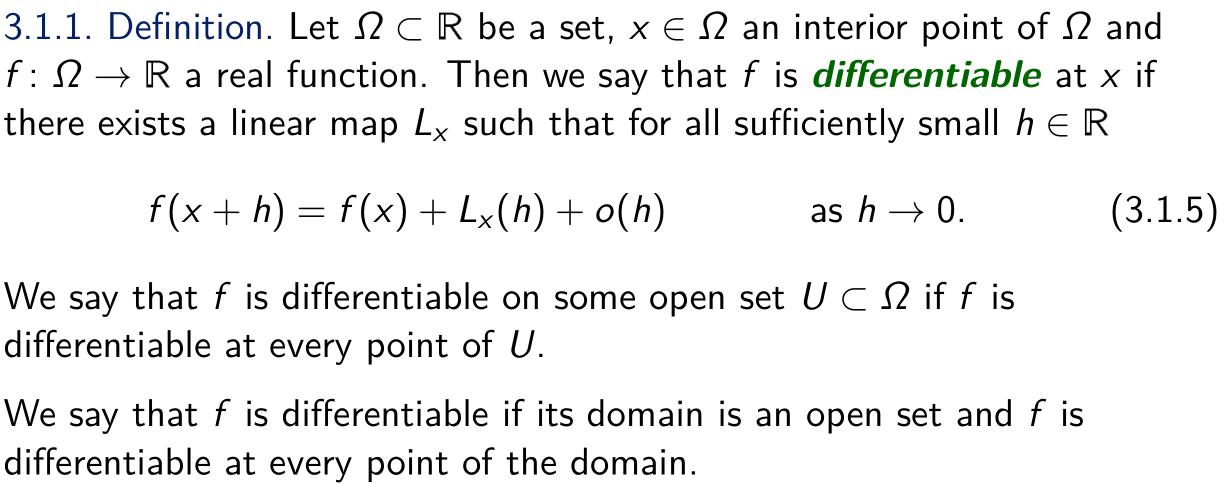
\includegraphics[width=0.9\textwidth]{2020-10-28-13-31-40.png}
    \end{figure}

    \question How to prove $L_x$ is unique if it exists?
    \nullspace
    \remark Due to the uniqueness of $L_x$, we define the derivative of $f$ at $x$: $$f'(x):=L_x$$
\end{frame}

\begin{frame}
    \frametitle{Derivative}
    \begin{figure}[H]
        \centering
        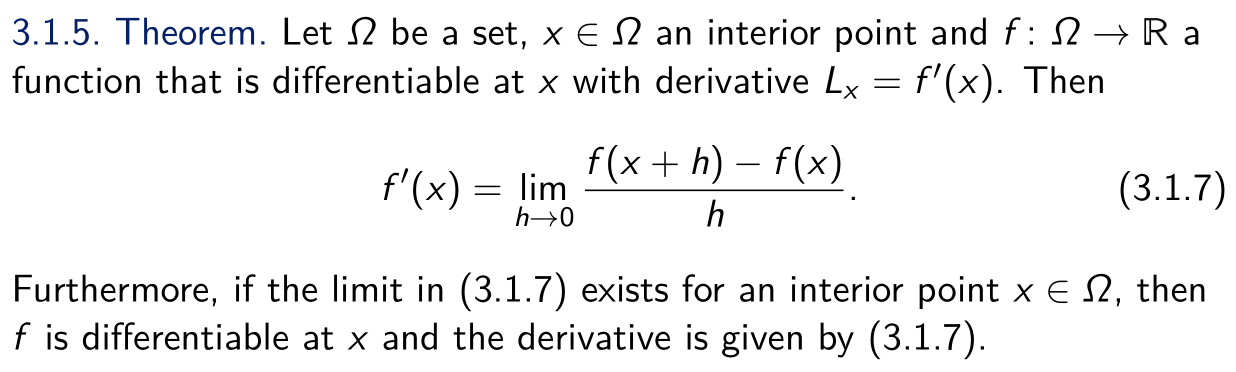
\includegraphics[width=0.9\textwidth]{2020-10-28-14-34-43.png}
    \end{figure}
    \textbf{Remark:} This theorem makes use od the geometric meaning of derivative (slope). However, I do \textbf{not} recommend you to remember the concept of derivate using slope. Because the concept of slope in high-dimension space is quite vague and non-intuitive while ``linear approximation'' remains to be meaningful in such a case.
\end{frame}

\begin{frame}
    \frametitle{Check Your Understanding}
    True of False?
    \begin{itemize}
        \item $L_x$ is essentially a number for a fixed $x\in\Omega$, because $L_x=\alpha$.
        \item The derivate of $f$ at $x$ is a line passing through $(x,f(x))$.
        \item For $f(x)=x^4,f'(x)=4x^3$, so $L_x$ may not be linear.
    \end{itemize}
    \pause
    Explanation:
    \begin{itemize}
        \item False. $L_X$ is essentially a linear map (function) rather than a real number. We abuse the notation of $L_x$ to represent $\alpha$. In fact, the notation $L_x=\alpha$ sometimes does not make sense. To remember that $L_x$ is a function, you can write $L_x:x\mapsto \alpha x$.
        \item False. The derivative of $f$ at $x$ is a linear map. Its graph does not necessarily pass $(x,f(x))$.
        \item False. This question is very tricky. Do not confuse \emph{derivative at some point} with \emph{function that gives derivative}. Fix $x=x_0$, $4x_0^3$ is just a real number. Therefore, the derivative at $x$ is a linear map $L_x:x\mapsto 4x_0^3\cdot x$. Essentially, $f'$ is a function that maps some point $x$ to the derivative of $f$ at $x$. i.e. $f':x\mapsto L_x$.
    \end{itemize}
\end{frame}

\begin{frame}
    \frametitle{Useful Result regarding Differentiation}

    \begin{enumerate}
        \item Linearity of differentiation
        \item Chain rule
        \item Product rule
        \item Quotient rule
    \end{enumerate}

\end{frame}

\begin{frame}
    \frametitle{Exercise}
    1. Find $f'(x)$, given $f(x)=g(x+g(x))+\dfrac{1}{g(x)}$. Assume $g(x)>0,g'(x)\neq 0$ exists.
    \nullspace
    2. Give an example of a function $f$ such that $\underset{x\to\infty}{\lim}f(x)$ exists, but $\underset{x\to\infty}{\lim}f'(x)$ does not exist.
    \nullspace
    3. Prove that if $\underset{x\to\infty}{\lim}f(x)$ and $\underset{x\to\infty}{\lim}f'(x)$ both exist, then $\underset{x\to\infty}{\lim}f'(x)=0$.
    \nullspace
    4. Suppose that $f$ is differentiable and $|f(x)-y(x)|\leq |x-y|^n$ for $n>1$. Prove that $f$ is constant.
\end{frame}

\begin{frame}
    \frametitle{End}
    \vspace{2.2cm}
    \begin{center}
        \Large
        Have Fun \\
        And \\
        Learn Well!\footnote[frame]{Special acknowledgement to former TA \textbf{Zhang Leyang}, who offered plenty of exercises and advice to my recitation class.}
    \end{center}
\end{frame}

\end{document}